%Material and methods

\section{Optimal experimental designs}
In the context of design of experiments (DOE), optimal designs are the holy grail that every experimenter want. However, researcher often use pre-made designs that fit a large amount of experiments instead of creating an optimal one. Since experimentations exist in all sizes and forms, not all pre-made designs are ideal. Therefore, creating an optimal design is a great choice to ensure that the design fits the experiment and not the other way around. In this section, we explain how and why we created a custom, optimal, design to fit our experiments.

\subsection{Orthogonal designs}
In design of experiments, orthogonal designs are interesting because they guarantees that each main effect and interaction can 
be estimated independently. Meaning that the effect of one factor or interaction can be estimated separately from the effect of 
other factors
and that the addition or subtraction of terms in the model does not affect the estimates.
In a regression or ANOVA-type model, the best linear unbiased predictor (or BLUE) of the regression coefficients is obtained by 
using 
the ordinary least squares (OLS) method, because it minimizes the variance of the estimators. 
These variances are often represented in variance-covariance (VCOV) matrix, 
where the diagonal is the variance of the estimators and the non-diagonal elements are the pairwise covariances between 
estimators. 
The inverse of this matrix is the information matrix, 
because it summarizes the available information  on the model's coefficients (a low variance means a lot of information, and 
inversely).
As detailed in \textcite{goos_optimal_2011}, when the information matrix is diagonal, then the design is said to be orthogonal.

\subsection{Optimality criteria}
In order to generate optimal designs, one needs to use an optimality criterion to compare different designs. 
The two main criteria are the D-optimality and the I-optimality. 
The first one aims at minimizing the variance of the factors effects estimates and is more useful for significance testing. 
D-optimal designs are therefore more appropriate for screening experiments. 
The second one aims at minimizing the average relative prediction variance over the experimental region. 
I-optimal designs are focused on prediction and thus are more suited to response surface experiments.
There also exists a G-optimality criterion that is similar to the I-optimality criterion but minimizes the maximum prediction 
variance. 
Recent work \parencite{rodriguez_generating_2010} has shown that I-optimal designs are often better choices than the G-optimal 
ones. 
Since this is a screening experiment, only the D-optimality is detailed here. 
For more information about I-optimal and G-optimal design, refer to \textcite{goos_optimal_2011,atkinson2014optimal}.

\subsubsection{D-optimality}
As said previously, for an orthogonal design all the non-diagonal elements of the VCOV matrix are null,
and thus, the determinant is simply the product of all the diagonal elements, i.e. the estimators variances.
Since the goal is to have the smallest variance of the estimates, the VCOV matrix with the smallest determinant will have the 
estimates with the smallest variance. 
Minimizing the determinant of the VCOV matrix is similar to maximizing the determinant of the information matrix. 
Therefore, the design with factor settings that maximize the determinant of information matrix, 
will maximize the available information about the model's parameters. 
This design is called the "D-optimal design", 
where the "D" stands for determinant and the value of the determinant itself is called the "D-optimality criterion".

For any model with two-levels factors and two-factor interaction effects, orthogonal designs will always be D-optimal. 
However if the number of runs is not a multiple of 4 then there are no orthogonal designs available for two-level factors. 
This condition offers little flexibility for experimenters and is not always feasible. 
In contrast, the optimal experimental design approach allows for any number of runs. 
However, in non-orthogonal designs the variance of the estimates is inflated and the estimates are correlated. 
Nevertheless this inflation is usually small and the correlation is too small to cause any concerns.
Therefore there exist non-orthogonal designs that still maximize the information of the model being estimated.
The D-optimal designs may not be unique. For a specified number of runs,
 several designs might have the maximal value for the determinant of the information matrix.\\


\subsection{Generating optimal designs}
In order to generate an optimal design, the determinant of the $\mathbf{X}^{\prime}\mathbf{X}$ matrix needs to be computed 
multiple times. 
Therefore algorithms are used to gain time and avoid errors. 
Several algorithms exist but the most common one is 
the coordinate exchange algorithm, created by \textcite{meyer_coordinate-exchange_1995}. 
It has the advantage to run in polynomial time, which means that the time needed to find an optimal design does not explode when 
the size of the design increases. 
Another similar algorithm is the point-exchange algorithm, created by \textcite{fedorov_theory_1972} and modified several times to speed 
it up \parencite{johnson_guidelines_1983,atkinson_construction_1989}. The main drawback of this algorithm is that it needs a list of 
possible design points as input, which can be quite tedious to do for large designs. In recent years, other types of algorithm 
such as genetic algorithms \parencite{heredia-langner_genetic_2003,heredia-langner_model-robust_2004}, simulating annealing algorithms 
\parencite{bohachevsky_generalized_1986,meyer_constructing_1988} and tabu search algorithms \parencite{jung_construction_1996} have 
been used in experimental designs. While these algorithms maintain a level of performance comparable to more traditional design 
construction techniques, they are not as popular because they are either far more complex, only feasible in some specific cases 
or better for some specific models and do not lead to designs that make a significant difference in practice.


\subsubsection{Coordinate-exchange algorithm}
The coordinate-exchange algorithm proceeds by iterating through the rows of the matrix of factors settings
\begin{equation}
\mathbf{D}= 
    \begin{bmatrix}
        x_{11} & x_{21} & \ldots & x_{k1} \\
        x_{12} & x_{22} & \ldots & x_{k2} \\
        \vdots & \vdots & \ddots & \vdots \\
        x_{1n} & x_{2n} & \ldots & x_{kn} 
    \end{bmatrix}
    \text{,}
    \label{mat:design_matrix}
\end{equation}
called the design matrix, of an experiment with $n$ runs and $k$ factors. The lines of this matrix essentially represent the 
coordinates of the runs in the experimental space, where each factor of the experiment is a dimension. This algorithm is called 
the coordinate-exchange algorithm, because in each iteration of the algorithm, possible changes for every element of the design 
matrix are considered. \\
It is straightforward to see that the design matrix $\mathbf{D}$ is a submatrix of the model matrix $\mathbf{X}$. It can happen 
the D-optimality criterion is zero. In those cases, the design is called singular and the inverse of the $\mathbf{X}^{\prime}
\mathbf{X}$ matrix does not exist. To avoid singularity, the number of design points (different rows in the design matrix $
\mathbf{D}$) must be greater than or equal to the number of model parameters.\\

The algorithm starts by generating a random design. For all continuous factors, the algorithm generates random values on the 
interval $[-1,+1]$. For all factors that are categorical, the algorithm randomly chooses a value in a discrete set of levels. 
This random starting design is almost always non-singular. If the design happens to be singular, then another new random 
starting design is computed.\\
In the next step, the algorithm improves the design on an element-by-element basis. For each element of the starting design, 
$x_{ij}$, a change to either $-1$ or $+1$ is considered, and its impact on the D-optimality criterion is evaluated. The change 
that increases the value of the D-optimality criterion the most, is kept. After investigating changes in each element of the 
design, the process is repeated until no element changes within an entire iteration through the factor settings or until a 
prespecified maximum number of iterations is reached. The obtained design is the best among a set of neighbouring designs but it 
is often a locally optimal design that is different for each random starting design. To select the best among all locally 
optimal designs, the algorithm is repeated a large number of times. The globally optimal design is then selected among all the 
locally optimal ones, as the one that yields the highest D-optimality criterion.

\subsection{Generating the design}
A custom design was created for the experimental set-up of the phenotyping platform, where the goal was to quantify the genotype 
and tank effect. Four factors were considered:

\begin{description}[align=left]
\item [Tank] In which tank was the plant situated (moving or still).
\item [Strip] Which of the 99 strip was used (1 to 99).
\item [Position] What was the position on the strip (1 to 5).
\item [Genotype] Which one of the 30 genotypes was used (1 to 30).
\end{description}

To fit the design, the design of experiment (DOE) tool was used in JMP. The four categorical factors were specified and 
\textit{Tank} and \textit{Strip} were set to "very hard to change" and "hard to change", respectively. Two whole plots of 99 
sub-plots each were specified to match the tanks and the strips. With 99 strips of five positions inside two tanks, 990 
experimental runs were available.\\
Initially the design was supposed to take into account the 99 different strips individually but the program couldn't converge to 
an optimal design because of its complexity. Instead only 33 strips were considered and the design was replicated 3 times to 
match the number of runs. Figures \ref{fig:moving_layout_30_geno} and \ref{fig:still_layout_30_geno}, display a schematic view 
of the design for the moving and still tank respectively.\\
The seeds were provided by the national institute of agronomic research (INRA) in Montpellier, France, as part of their own 
research on these historical series\footnote{Historical series correspond to varieties that have been cultivated and bred for 
some time, mainly due to their physiological specificities.}. They sent a total of 30 seeds per genotype and besides that, an 
extra 150 seeds of another genotype, called the "border genotype", was sent by the provider. The main utility of the border 
genotype is to fill the gaps left by non germinated seeds. Since, in this experiment, only 900 runs (30 genotypes x 30 seeds) 
were occupied, the border genotype was also be used to fill the 90 empty runs. Since this genotype is not part of the historical 
series, it was not considered in the design of the experiment.

\begin{sidewaysfigure}[ht]
    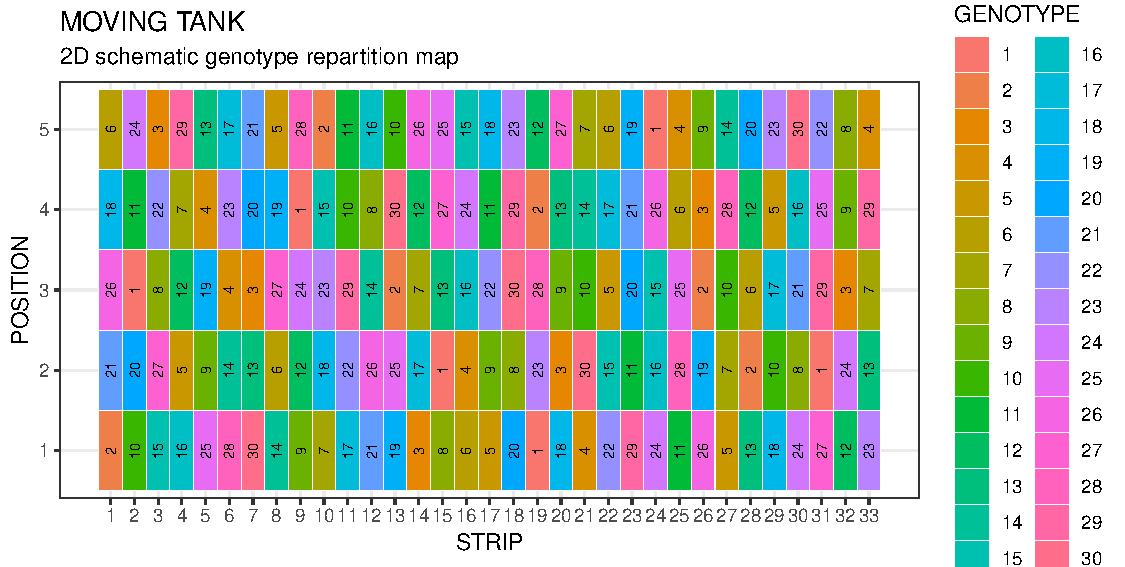
\includegraphics[width=\textwidth]{../../Figures/design_layout_moving.pdf} 
    \caption{2D schematic representation of the experimental design for 33 individual strips and 30 genotypes in the moving 
    tank.}
    \label{fig:moving_layout_30_geno}
\end{sidewaysfigure}

\begin{sidewaysfigure}[ht]
    \includegraphics[width=\textwidth]{../../Figures/design_layout_still.pdf} 
    \caption{2D schematic representation of the experimental design for 33 individual strips and 30 genotypes in the still 
    tank.}
    \label{fig:still_layout_30_geno}
\end{sidewaysfigure}

\subsection{Design's characteristics}


\section{Phenotyping experiment}
The phenotyping experiment took place between February 25th and March 13th. The seeds were first germinated and then transferred 
onto the platform. After the end of the experiment the plants were weighted, dried and weighted again to obtain dry and fresh 
weight.

\subsection{Germination}
Previous experiments in the greenhouses showed that germination of maize seeds on the platform often lead to asphyxiation of the 
seeds. 
Because of this, the seeds were germinated in an outside germination chamber and were only transferred onto the platform once 
germinated.

The seeds were placed in a temperature-controlled room at 20$^{\circ}$C for 3 days, inside a germination chamber. The chamber consisted of 2 PVC trays to which an air-fog machine was connected, to keep the seeds moist. 
Inside each tray, PVC plates were disposed diagonally and evenly spaced (fig. \ref{fig:germination_chamber_diagram}). On those plates, the seeds were arranged on a filtering paper sheet with ledges to support the weight of the seeds (figure \ref{fig:germiantion_ledge} and figure \ref{fig:photo_germination_plate}). The bottom of the trays were filled with water to keep the filtering paper moist. 
There were 17 plates in total, 15 for the 30 genotypes and 2 for the border genotype (150 seeds dispatched on 2 plates). 

    \begin{figure}[!htb]
        \centering
        \begin{subfigure}[b]{0.95\textwidth}
            \centering
            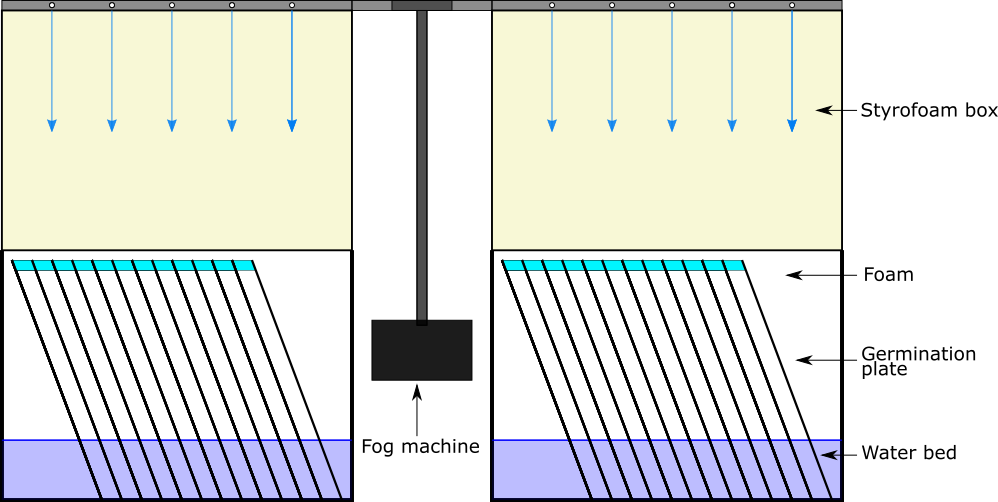
\includegraphics[width=\textwidth]{figures/germination_chamber_diagram.png}
            \caption[]%
            {Global schematic view of the germination chamber: a fog machine assure constant humidity in the germination 
            chambers by creating fog at regular intervals (the blue arrows represent the path of the fog). The plates are placed 
            at a 60$^{\circ}$ angle and 5 cm apart}    
            \label{fig:germination_chamber_diagram}
        \end{subfigure}
        \vskip\baselineskip
        \begin{subfigure}[b]{0.475\textwidth}   
            \centering 
            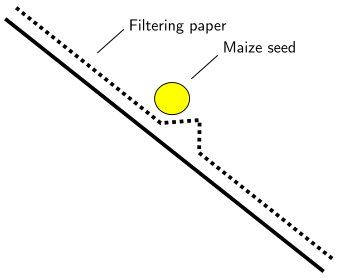
\includegraphics[width=\textwidth]{figures/germination_ledge.png}
            \caption[]%
            {Schematic view of a germination ledge on a PVC plate: each seed is fixed in position on the ledge by an additional 
            drop of agar solution to avoid any fall-off}    
            \label{fig:germiantion_ledge}
        \end{subfigure}
        \quad
        \begin{subfigure}[b]{0.475\textwidth}   
            \centering 
            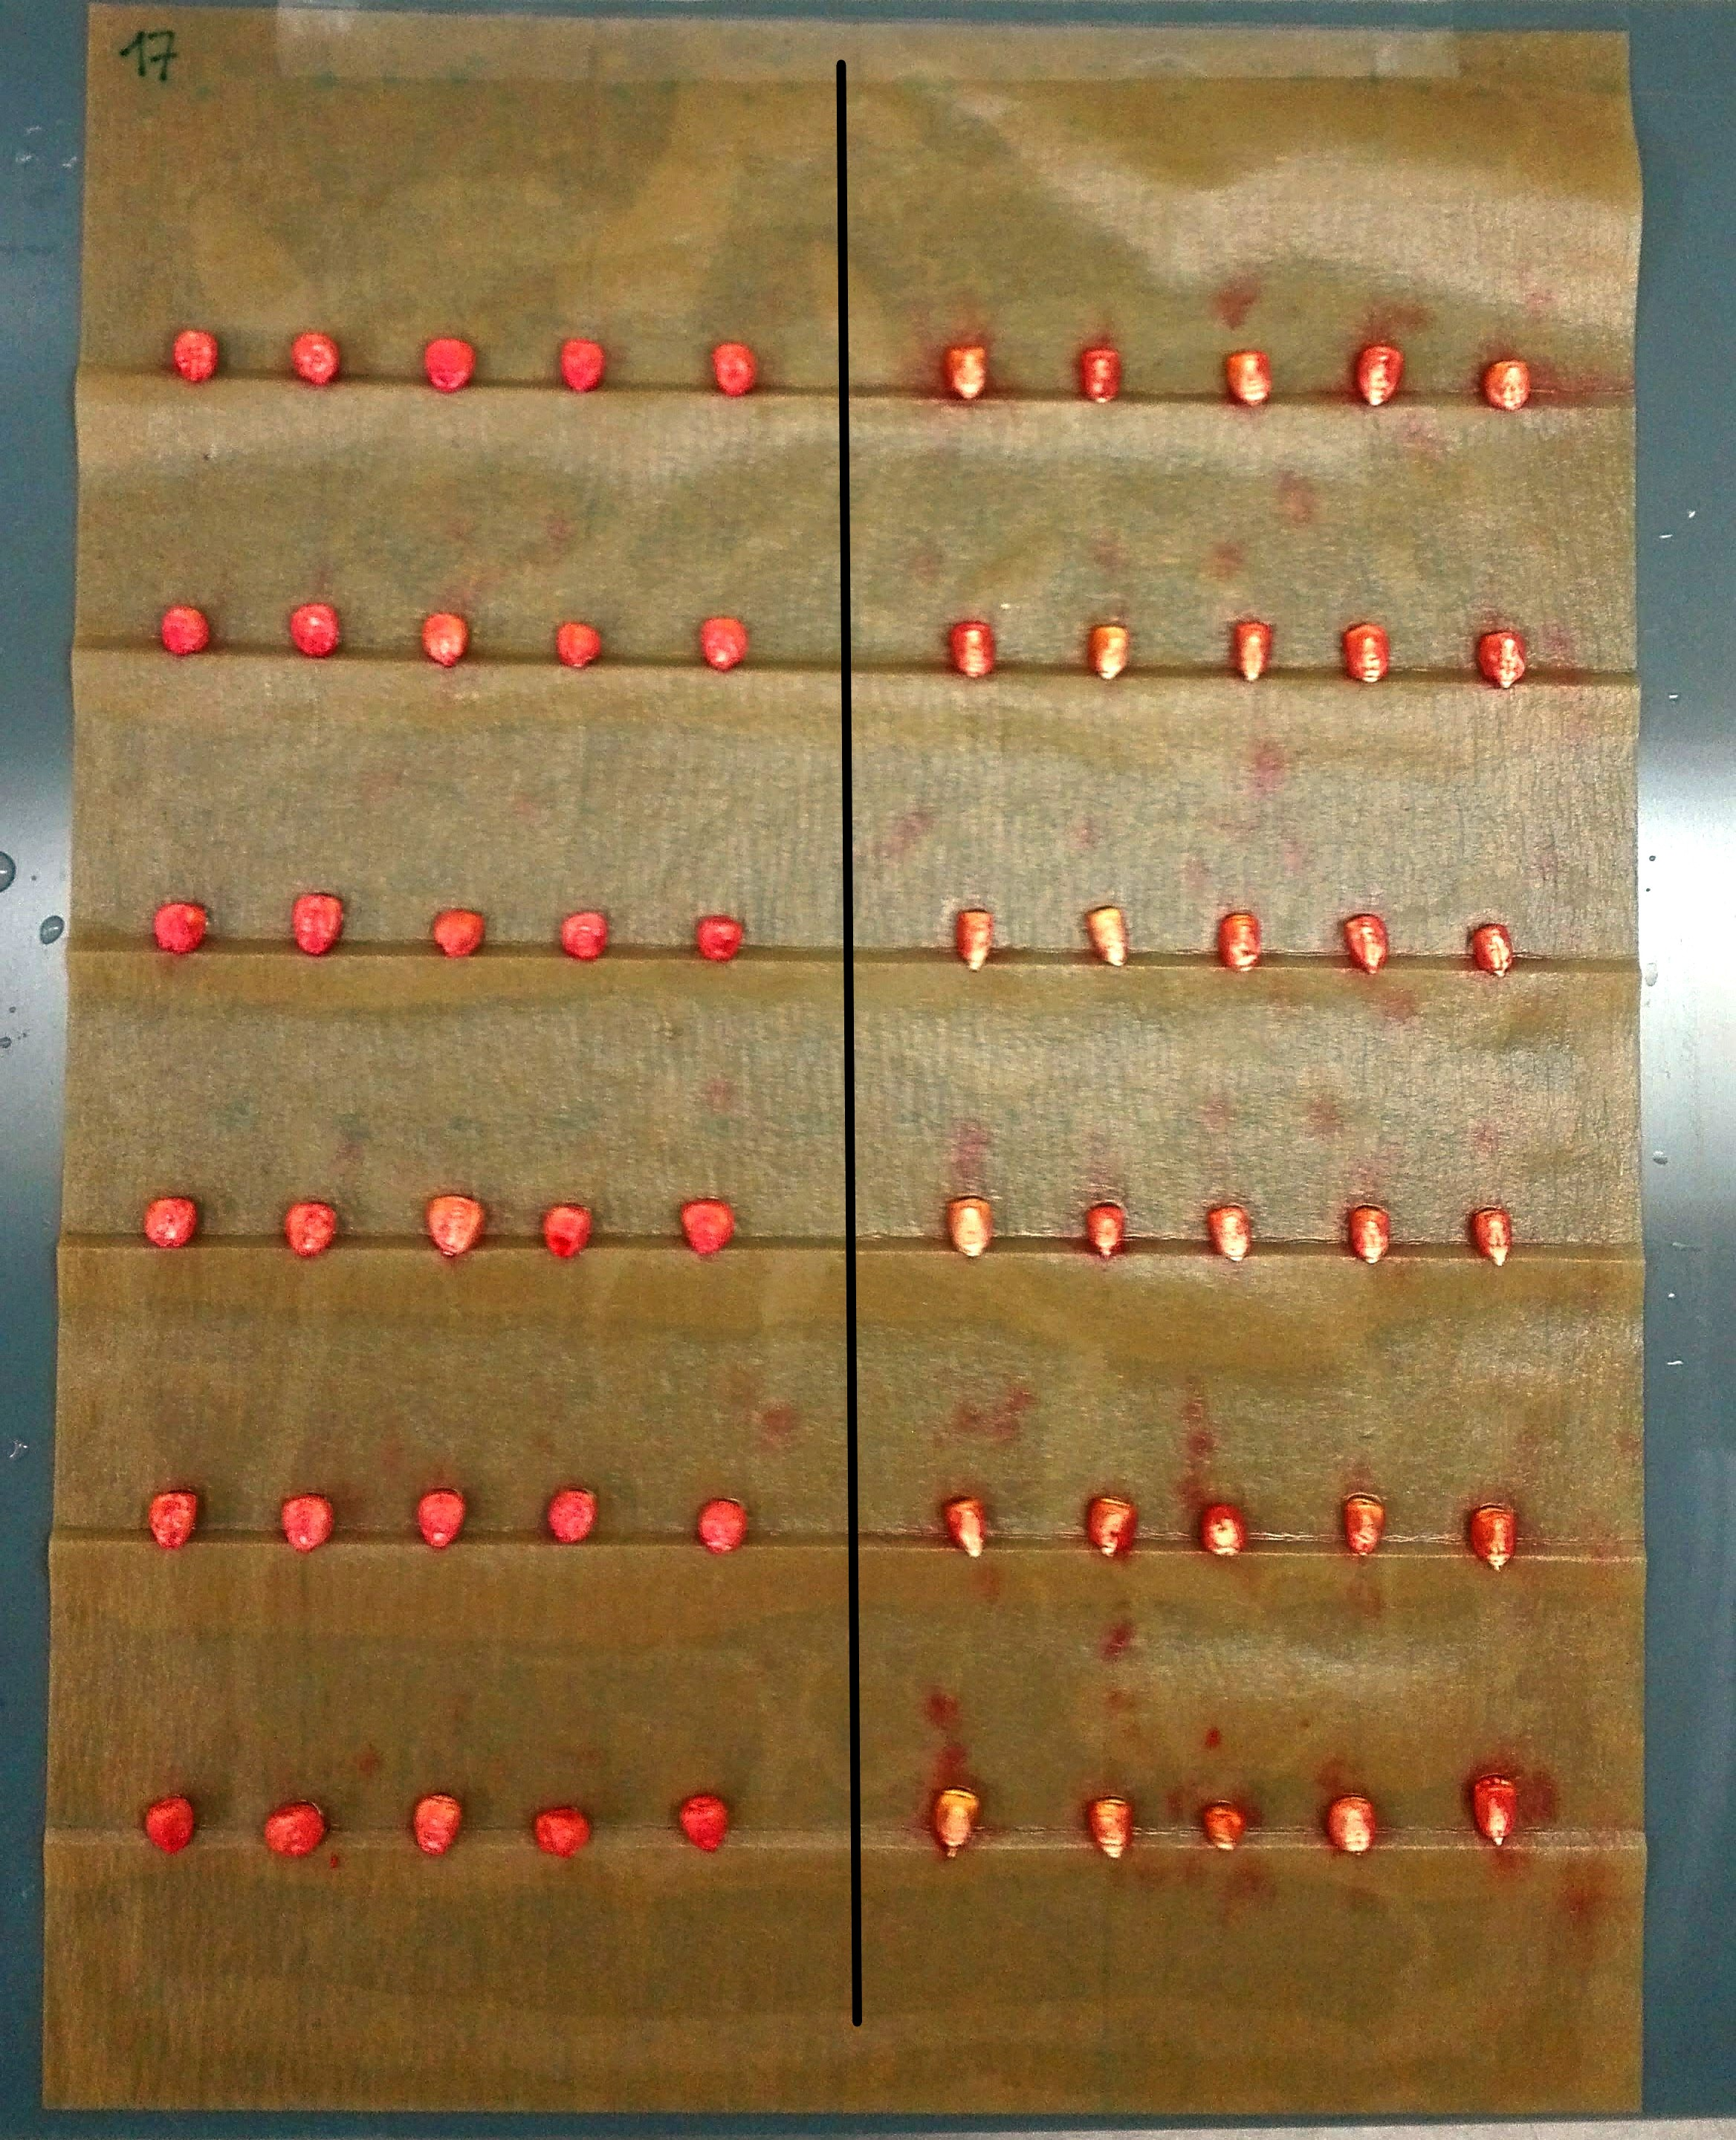
\includegraphics[width=\textwidth]{figures/photo_germination_plate.jpg}
            \caption[]%
            {30 cm by 40 cm PVC plate with seeds on filtering paper (the black line represents the separation between the two 
           genotypes on the plate). Each sheet had 6 rows of 10 seeds with one genotype on the left and one genotype on the 
           right.}    
            \label{fig:photo_germination_plate}
        \end{subfigure}
        \caption{Germination chamber diagram with detailed view and pictures}
    \end{figure}

After 3 days into the chamber, not all seeds were germinated, table \ref{tab:germination_percentage} presents the germination 
rates and mean seed weights for all the genotypes used (including the border genotype). The non-germination was mainly due to 
the fact that seeds fell into the water bed and because mold grew on some filtering paper.

%table for the germination rates after the outside germination process

\begin{table}[ht]
\centering
\caption[Germination rates and seed weights]{Germination rate and mean seed weight for each genotype used. (there is no data concerning the germination rate of the 
border genotype because it was not measured).}

\rowcolors{2}{gray!25}{white}

\begin{tabular}{lcc}
  \toprule
  %\rowcolor{gray!50}
Genotype & Germination rate (\%) & Mean seed weight (g) \\ 
  \midrule
1 & 80.00 & 0.28 \\ 
  2 & 86.67 & 0.36 \\ 
  3 & 96.67 & 0.36 \\ 
  4 & 73.33 & 0.28 \\ 
  5 & 100.00 & 0.32 \\ 
  6 & 96.67 & 0.24 \\ 
  7 & 96.67 & 0.19 \\ 
  8 & 70.00 & 0.31 \\ 
  9 & 96.67 & 0.33 \\ 
  10 & 96.67 & 0.25 \\ 
  11 & 60.00 & 0.33 \\ 
  12 & 93.33 & 0.27 \\ 
  13 & 90.00 & 0.24 \\ 
  14 & 86.67 & 0.31 \\ 
  15 & 56.67 & 0.35 \\ 
  16 & 90.00 & 0.28 \\ 
  17 & 90.00 & 0.30 \\ 
  18 & 86.67 & 0.26 \\ 
  19 & 100.00 & 0.26 \\ 
  20 & 86.67 & 0.28 \\ 
  21 & 86.67 & 0.32 \\ 
  22 & 53.33 & 0.30 \\ 
  23 & 73.33 & 0.28 \\ 
  24 & 100.00 & 0.16 \\ 
  25 & 96.67 & 0.19 \\ 
  26 & 96.67 & 0.25 \\ 
  27 & 96.67 & 0.28 \\ 
  28 & 83.33 & 0.36 \\ 
  29 & 93.33 & 0.30 \\ 
  30 & 73.33 & 0.35 \\ 
  31 & / & 0.38 \\ 
   \bottomrule
\end{tabular}
\label{tab:germination_percentage}
\end{table}

\subsection{Phenotyping platform}
The phenotyping platform is located inside a greenhouse in the facilities of the UCLouvain (Louvain-la-Neuve, Belgium). 
It consists of two aeroponic tanks on which are arranged 99 styrofoam strips, each with five holes. 
At the end of each tank is a high definition camera that scans the root system of each plant individually, when it passes in 
front of it (fig. \ref{fig:tank}). 
The strips rotate in a clockwise fashion in the tank and a full rotation is completed in 2 hours. 
Three sprinklers are placed regularly at the bottom of each side of the tank (fig. \ref{fig:tank_transversal_view}). 
The sprinklers spray nutrient solution\footnote{The precise concentration of the Hoagland solution is presented in appendix 
\ref{appendix:hoagland}} at regular intervals, set by the operator. 
The spraying pattern (interval and duration) can be differentiated between day and night and can be modified at any moment of 
the experiment.
In this case the patterns were 5 seconds of spraying ever 295 seconds all the time.
During the experiment, the temperature of the greenhouse was set to 20$^{\circ}$C at day and 18$^{\circ}$C at night and the 
lights were on from 6 AM to 10 PM. 
At the start of the experiment seeds were placed inside a foam cork and then placed inside a hole on a strip (fig 
\ref{fig:seed_platform_close_up}). 
They were placed at the bottom to allow the root system to grow freely. 
The corks are drilled vertically to let the leaf system develop with less resistance and allow a direct access to sunlight. 
More information about the platform is available in appendix \ref{appendix:platform_info}.

After 3 days in the germination chamber, the germinated seeds were transferred onto the platform following the created design, and the non-germinated seeds were discarded. The first tank was constantly moving but only scanning the root systems once a day, while the second tank was only moving once a day to scan the root system of the plants and stayed still the rest of the day.

\begin{figure}[!htb]
        \centering
        \begin{subfigure}[b]{0.95\textwidth}
            \centering
            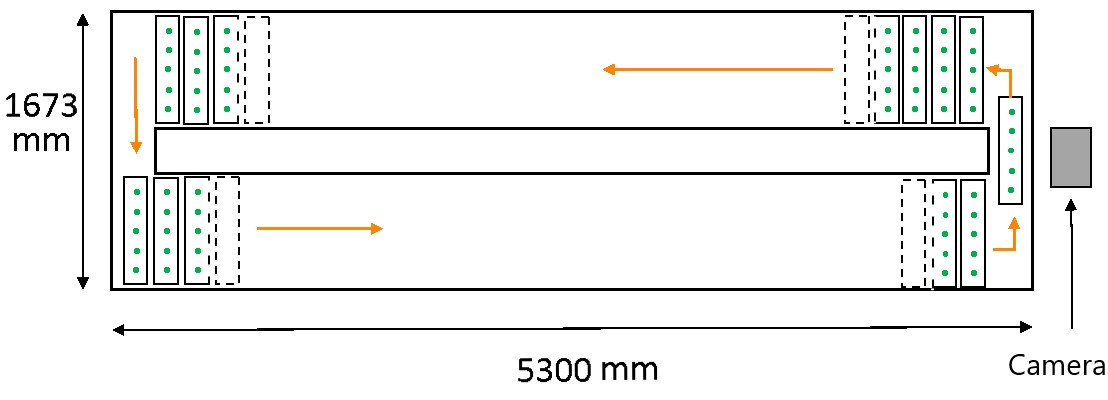
\includegraphics[width=\textwidth]{figures/tank.jpg}
            \caption{Schematic view of an aeroponic tank: plants are hold on strips, 5 plants per strip (green dots on layout). There are 99 strips in the tank for a total of 495 plants/tank. Strips move in the direction indicated by orange arrows}    
            \label{fig:tank}
        \end{subfigure}
        \vskip\baselineskip
        \begin{subfigure}[b]{0.475\textwidth}   
            \centering
            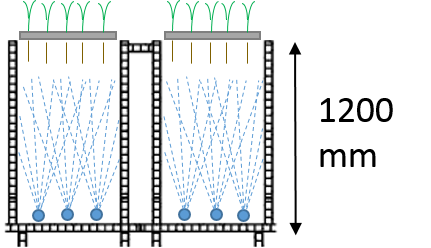
\includegraphics[width=\textwidth]{figures/tank_transversal_view.png}
            \caption{Transversal schematic view of an aeroponic tank of the platform: at the bottom of each tank, sprinklers (represented in blue in the layout) are disposed at regular interval and spray nutritive solution}    
            \label{fig:tank_transversal_view}
        \end{subfigure}
        \quad
        \begin{subfigure}[b]{0.475\textwidth}   
            \centering
            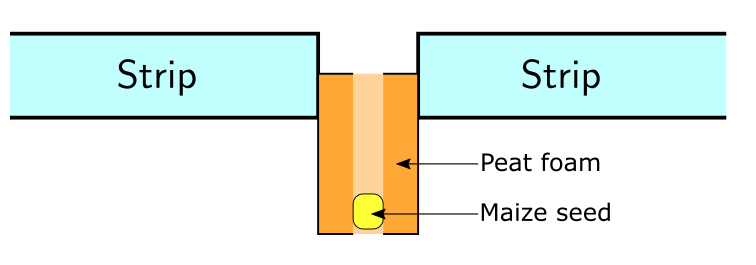
\includegraphics[width=\textwidth]{figures/seed_platform_close_up.png}
            \caption{Close up schematic view of a strip: inside each hole, seeds are placed inside a pierced peatfom cork to allow the root system to develop frelly}    
            \label{fig:seed_platform_close_up}
        \end{subfigure}
        \caption{Detailed diagrams about the phenotyping platform}
    \end{figure}


\section{Data processing}
After 15 days, the plants were considered fully grown and the experiment was stopped. The leaf and root systems were separated and weighted individually on scales precise to 0.001 g. They were then dried for 3 days in a 70$^{\circ}$C oven. After the drying process, they were weighted again. For each plant, the remaining of the seed was consistently kept on the root system.
Two kind of data were obtained from the experiment: weight data (dry and fresh) of the fully grown plants and root scan data. Five variables were kept for the spatial analysis:

\begin{itemize}
\item $FRESH\_RS$: fresh weight of the root system
\item $FRESH\_LS$: fresh weight of the leaf system
\item $DRY\_RS$: dry weight of the root system
\item $DRY\_LS$: dry weight of the leaf system
\item $AREA$: percentage of the total area occupied by the root system
\end{itemize} 

To be used as inputs in the models, those data need to be processed. The following sections details this step.

\subsection{Weight data}
For some plants, the germinated seeds placed on the platform did not fully grow or had an abnormal growth, but all the plants were still weighted to avoid leaving out any data. Therefore some data points need to be handled more carefully, as they do not represent the genotype's growth correctly. However, a correct growth, representative of the genotype, is hard to define because the influence of the conditions on each genotype is unknown. Therefore, instead of choosing which plants are outliers in a binary way, we attributed weights to each plant to express the quality of the data. Those weights were established by reviewing the final root scan of each plant and checking the different factors that could have an influence. The factors chosen are the following:

\begin{itemize}
\item $NO\_RS$: no additional root to the primary root
\item $NO\_LS$: no visible leaf system 
\item $BAD\_LS$: leaf system grew under the strip (or abnormally in general)
\item  $NO\_SEED$: no seed (or an empty cork) present on this position
\item $NOT\_FG$: plant not fully grown
\item $OVERLAP$: leaf (or root) system of another plant overlaps on the root scan
\item $OK$: no influential factors
\end{itemize} 

An visualization of those factors with example pictures is presented in figure \ref{fig:example_influential_factors}. Some plants were attributed several influential factors, but $OK$, $NO\_SEED$ and $NOT\_FG$ were considered as exclusive. The factor attribution was ambiguous for some pictures, in those cases the plant were considered $OK$ to avoid losing any data points.
Following the determination of the factors, weights were attributed to each variable according to the weight matrix, presented in table \ref{tab:weight_attribution_matrix}.


% Table generated by Excel2LaTeX from sheet 'weights'
\begin{table}[htbp]
  \centering
  \caption[Weight attribution matrix]{Weight attribution matrix for the different factors and variables. LS weight is both the fresh and dry weight for leaf system and RS weight is the same for the root system}
  	\rowcolors{2}{gray!25}{white}
    \begin{tabular}{lrrr}
    \toprule
    CODE  & LS weight & RS weight & Area \\
    \midrule
    NO\_RS & 1     & 1     & 1 \\
    NO\_LS & 2     & 2     & 2 \\
    BAD\_LS & 3     & 3     & 3 \\
    NOT\_FG & 4     & 4     & 4 \\
    NO\_SEED & 0	& 0		& 0 \\
    OK 		& 5 	& 5 	& 5 \\
    OVERLAP & 5     & 5     & 0 \\
    \bottomrule
    \end{tabular}%
  \label{tab:weight_attribution_matrix}%
\end{table}%


\begin{sidewaysfigure}[ht]
\centering
\begin{subfigure}[t]{.13\textwidth}
  \centering
  \includegraphics[width=\linewidth]{figures/NO_RS.jpg}
  \caption{$NO_RS$: no additional root, other than the primary}
  \label{fig:NO_RS}
\end{subfigure}
%
\begin{subfigure}[t]{.13\textwidth}
  \centering
  \includegraphics[width=\linewidth]{figures/NO_LS.jpg}
  \caption{$NO\_LS$: no apparent leaf system}
  \label{fig:NO_LS}
\end{subfigure}
%
\begin{subfigure}[t]{.13\textwidth}
  \centering
  \includegraphics[width=\linewidth]{figures/BAD_LS.jpg}
  \caption{$BAD\_LS$: the leaf system grew under the strip and deviated to the right (obstruction of another plant)}
  \label{fig:BAD_LS}
\end{subfigure}
%
\begin{subfigure}[t]{.13\textwidth}
  \centering
  \includegraphics[width=\linewidth]{figures/NO_SEED.jpg}
  \caption{$NO\_SEED$}
  \label{fig:NO_SEED}
\end{subfigure}
%
\begin{subfigure}[t]{.13\textwidth}
  \centering
  \includegraphics[width=\linewidth]{figures/NOT_FG.jpg}
  \caption{$NOT\_FG$: both system are present but underdeveloped compared to other images }
  \label{fig:NOT_FG}
\end{subfigure}
%
\begin{subfigure}[t]{.13\textwidth}
  \centering
  \includegraphics[width=\linewidth]{figures/OVERLAP.jpg}
  \caption{$OVERLAP$: the leaf system of another plant hides the root system of the plant}
  \label{fig:OVERLAP}
\end{subfigure}
%
\begin{subfigure}[t]{.13\textwidth}
  \centering
  \includegraphics[width=\linewidth]{figures/OK.jpg}
  \caption{$OK$, the green box represents the bounding area for the computation of the root area}
  \label{fig:OK}
\end{subfigure}
%
\caption{Example pictures of the influential factors chosen for the weight attribution.}
\label{fig:example_influential_factors}
\end{sidewaysfigure}

\subsection{Root pictures}
The area of the root system was computed using the final root scan of each plant. Each picture was converted to gray-scale, resized to a specific bounding rectangle and binarized. The bounding box is illustrated on figure \ref{fig:OK}. The threshold for the binarization was 140 on a 0 to 255 scale. Since the roots are black on the original picture, the binarization was completed without any issues. The area of the root system was expressed as a percentage of the total area of the bounding box, by counting the black pixels in the image. All the processing was done in python using the opencv package.


\section{SpATS model}
In this section, the SpATS model is introduced. For a more thorough treatment of the model and all its components, see \textcite{rodriguez-alvarez_spatial_2016}.\\
Consider a field trial of $n$ plots arranged in a rectangular grid, where the plot positions are collected in vectors of row $(\mathbf{r})$ and column $(\mathbf{c})$ coordinates. If $\mathbf{y}$ is the vector of plot data in field order, a common model for $\mathbf{y}$, to use as a starting point is
	\begin{equation}
	    \boldsymbol{y}=\mathbf{1}_{n} \beta_{0}+\boldsymbol{Z}_{r} \boldsymbol{c}_{r}+\boldsymbol{Z}_{c} \boldsymbol{c}_{c}
	    +\varepsilon
	\end{equation}
were $\mathbf{1}_{n}$ is a column-vector of ones of length $n$, $\boldsymbol{c}_{r}$ and $\boldsymbol{c}_{c}$ are, respectively, the random effect coefficients for the rows and columns and associated matrix $\boldsymbol{Z}_{r}$ and $\boldsymbol{Z}_{c}$. To fully capture complex spatial patterns, a smooth bivariate surface jointly defined over the row and column positions is added to the model, which becomes
	\begin{equation}
	    \boldsymbol{y}=f(\boldsymbol{u}, \boldsymbol{v})+\boldsymbol{Z}_{r} \boldsymbol{c}_{r}+\boldsymbol{Z}_{c} \boldsymbol{c}
	    _{c}+\boldsymbol{\varepsilon}
	    \label{eq:base_model_bismooth_surface}
	\end{equation}
where $\mathbf{u}$ and $\mathbf{v}$ are, respectively, the vector of row and columns positions and where $f(.,.)$ represents the smooth bivariate function. Note that the intercept term, $\beta_0$ is embedded into $f(u,v)$. To better understand this function, let us decompose it in a nested-ANOVA structure
	\begin{align}
	f ( \boldsymbol { u } , \boldsymbol { v } ) & = \underbrace { \mathbf { 1 } _ { n } \beta _ { 0 } + \boldsymbol { u } \beta
	 _ { 1 } + \boldsymbol { v } \beta _ { 2 } + \boldsymbol { u } \odot \boldsymbol { v } \beta _ { 3 } } _ { \text { Bilinear
	  polynomial } } \nonumber \\
	 & + \underbrace { f _ { u } ( \boldsymbol { u } ) + f _ { v } ( \boldsymbol { v } ) + \boldsymbol { u } \odot h _ { v } (
	  \boldsymbol { v } ) + \boldsymbol { v } \odot h _ { u } ( \boldsymbol { u } ) + f _ { u , v } ( \boldsymbol { u } ,
	   \boldsymbol { v } ) }_{\text{Smooth part}}
	 \label{eq:full_bivariate_smooth_surface_model}
	\end{align}
where $\odot$ denotes the element-wise matrix product\footnote{See appendix \ref{appendix:add_info} for details about the element-wise matrix product.}. There are now two components to the model: a bilinear polynomial part(parametric) and a smooth part (non-parametric). The parametric part includes the linear trends along rows ($\beta_1$) and columns ($\beta_2$) as well as a linear interaction trend ($\beta_3$). The smooth part models the deviation from the compound linear trend, and can be decomposed in the following elements:
	\begin{itemize}
		\item $f_{u}(\boldsymbol{u})$  is a smooth trend along the rows, identical for all columns (i.e., a main smooth effect).
		\item $f_{v}(\boldsymbol{v})$ is a smooth trend along the columns, identical for all rows.
		\item $\boldsymbol{v} \odot h_{u} (\boldsymbol{u})$ and $\boldsymbol{u} \odot h_{v} (\boldsymbol{v})$ are linear-by-
		smooth interaction trends. For instance, $\boldsymbol{u} \odot h_{v}(\boldsymbol{v})$ is a varying coefficient surface 
		trend, consisting of functions, linear in the rows, for each column, but with slopes that change smoothly along the 
		columns, $h_{v}boldsymbol{v})$.
		\item $f_{u,v}(\boldsymbol{u},\boldsymbol{v})$ is a smooth-by-smooth interaction trend jointly defined over the row and 
		column directions.
	\end{itemize}
In total, six components are used to model the surface $f$. This may seem like a lot but this allows the translation of model \ref{eq:base_model_bismooth_surface} into a standard mixed model. An interesting property of this proposal is that since $u$ and $v$ are row and column position, it allows depicting the spatial trend in a grid finer than the number of rows and columns. Figure \ref{fig:bilinear_and_smooth_decomposition} shows an example of those six components in the context of a barley uniformity performed by \textcite{williams1988contemporary}. It shows clearly how the additional components, help to capture small variations in the spatial data.

\begin{figure}[hbtp]
\centering
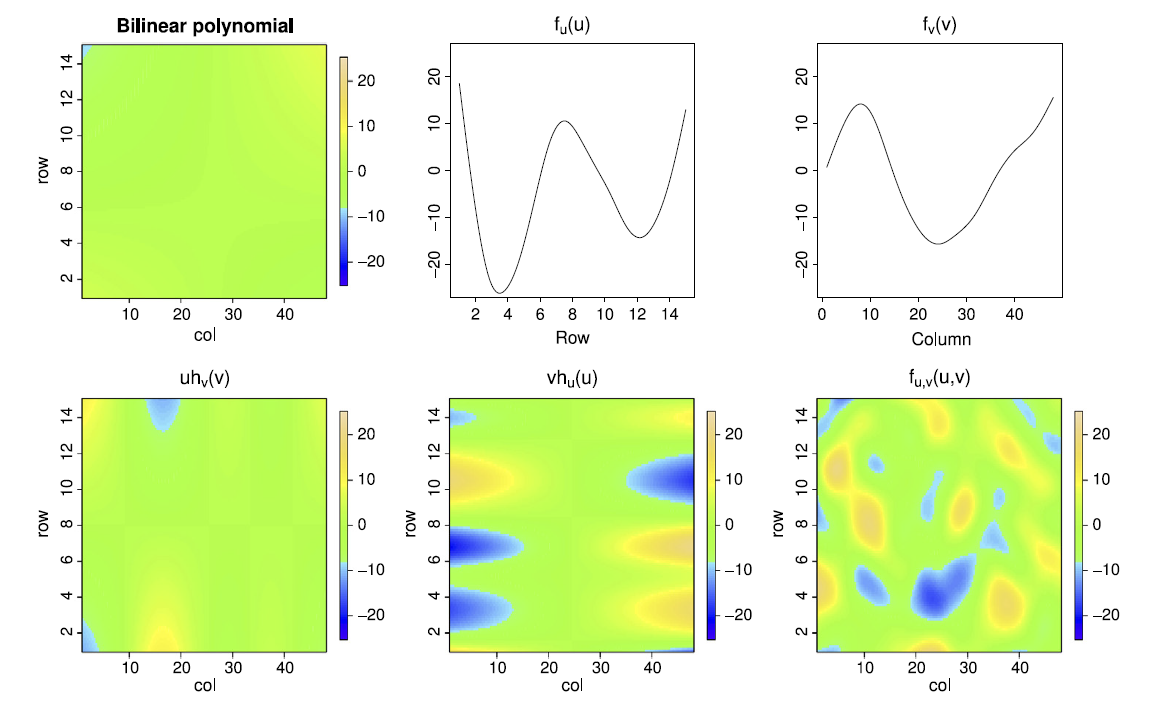
\includegraphics[width=\textwidth]{../figures/bilinear_polynomial.PNG}
\caption[Bilinear and smooth components of the PS-ANOVA decomposition]{Bilinear and smooth components of the PS-ANOVA decomposition of the estimated spatial trend for the barley uniformity
data from \textcite{rodriguez-alvarez_correcting_2018}.}
\label{fig:bilinear_and_smooth_decomposition}
\end{figure}


\subsection{Modelling using P-splines}
The functions $f_u$, $f_v$, $h_u$ and $h_v$ are constructed  with variations on one-dimensional P-splines, while $f_{u,v}$ is based on tensor products P-splines.\\
For clarity's sake, let us consider a model only containing a smooth bivariate surface and an error term
	\begin{equation}
	    y _ { i } = f \left( u _ { i } , v _ { i } \right) + \varepsilon _ { i } , \text { with } \varepsilon _ { i } \sim N 
	    \left( 0 , \sigma ^ { 2 } \right) \text{.}
		\label{eq:smooth_part_only_model}
	\end{equation}
\textcite{lee_efficient_2013} show that it can be represented using B-splines\footnote{See appendix \ref{appendix:add_info} for details about B-splines and P-splines.}. Let us form two B-splines basis:
\begin{enumerate}
\item one for the columns, $\boldsymbol{\invbreve{B}}$ with $ b_{il}= \invbreve{B}_l(u_i)$, where $\invbreve{B}_l(u_i)$ is the $l$th B-spline of the basis, evaluated at $u_i$
\item and one for the rows, $\boldsymbol{\breve{B}}$ with $ b_{ip}= \breve{B}_p(v_i)$, where $\breve{B}_l(v_i)$ is the $p$th B-spline of the basis, evaluated at $v_i$.
\end{enumerate}
Then, the smooth-by-smooth interaction can be written using those basis
\begin{equation}
	f \left(u_{i},v_{i}\right)=\sum_{l=1}^{L}\sum_{p=1}^{P}\invbreve{B}_{l}\left(u_{i}\right)\breve{B}_{p}\left(v_{i}\right) 
	\alpha_{lp}\text{,}
\end{equation}
where $\boldsymbol{\alpha} = (\alpha_{11},\ldots,\alpha_{1P},\ldots,\alpha_{LP})^t$ is a vector of unknown regression coefficients of dimension $(LP \times 1)$. Note that $\boldsymbol{\invbreve{B}}$ and $\boldsymbol{\breve{B}}$ are matrices of order $n \times L$ and $n\times P$ respectively, where $L$ and $P$ are the number of the B-spline basis functions. \textcite{dierckx_curve_1995} shows that, in the P-spline framework, the smooth-by-smooth interaction $f(u_i,v_i)$ is modelled by the tensor product of B-splines bases. Then, we can write, in matrix notation,
\begin{equation}
    \boldsymbol{B} = \boldsymbol{\invbreve{B}} \boxdot \boldsymbol{\breve{B}} = \left( \boldsymbol{\invbreve{B}} \otimes
    \boldsymbol{1} _ { L } ^ { t } \right) \odot \left( \mathbf { 1 } _ { P } ^ { t } \otimes \boldsymbol{\breve{B}} \right)
    \text{,}
\end{equation}
where the operation $\boxdot$ is defined in terms of the Kronecker product of two matrices (denoted by $\otimes$) and the 
element-by-element multiplication of two matrices (denoted by $\odot$)\footnote{See appendix \ref{appendix:add_info} for details 
about the Kronecker, and the element-wise products}. Therefore model (\ref{eq:smooth_part_only_model}) can be written in matrix 
notation:

\begin{equation}
    \boldsymbol{y} = \boldsymbol{B}\boldsymbol{\alpha} + \boldsymbol{\epsilon}
    \text{.}
    \label{eq:spline_model_mat_form}
\end{equation}

The coefficients of this parametric model can be estimated by minimizing the sum of squares. The explicit solution is then:
\begin{equation}
	\Hat{\boldsymbol{\alpha}} = (\mathbf{B}^t\mathbf{B})^{-1}\mathbf{B}^t\mathbf{y}
\end{equation}
To prevent over-fitting, 
\textcite{eilers_flexible_1996} propose to incorporate a discrete penalty on the coefficient associated to adjacent B-splines.
As described in details in appendix \ref{appendix:polynomial_splines}, this penalty also determines the smoothness of the 
splines. The solution of equation \ref{eq:spline_model_mat_form} then becomes 
\begin{equation}
    \widehat{\boldsymbol{\alpha}}=\left(\boldsymbol{B}^{t} \boldsymbol{B}+\boldsymbol{P}\right)^{-1} \boldsymbol{B}^{t} 
    \boldsymbol{y}
    \text{,}
\end{equation}
where $\boldsymbol{P}$ is the penalty matrix. The details of this solution are presented in appendix 
\ref{appendix:penalized_solution_form}, but the important point to remember here, is that the smoothness of the bivariate 
surface is defined by the penalty matrix, which only depend on two tuning parameters  $\invbreve{\lambda}$ (smoothing along the 
columns) and $\breve{\lambda}$ (smoothing along the rows).

\subsection{Mixed model based smoothing parameter selection}

As explained in \textcite{rodriguez-alvarez_spatial_2016}, $\mathbf{P}$ is rank-deficient, meaning that the rank is smaller than the 
number of rows and/or columns, and this causes numerical instability when applying mixed model estimation techniques. To obtain 
a full-rank penalty matrix, the key is to write model \ref{eq:spline_model_mat_form} as 
\begin{equation}
    \mathbf{B}\boldsymbol{\alpha} = \boldsymbol{X}_{s} \boldsymbol{\beta}_{s}+\boldsymbol{Z}_{s} \boldsymbol{c}_{s}
    \text{.}
\end{equation}
There are now two bases: $\mathbf{X}_{s}$, with coefficients that are not penalized at all, and $\mathbf{Z}_{s}$, with a size 
penalty on its coefficients. This decomposition follows the proposal by \textcite{lee_p-spline_2011}, based on eigenvalue 
decomposition which gives rise to a diagonal penalty matrix.\\
The two bases have the following structures:
\begin{equation}
    \boldsymbol{X}_{s}=\left[\mathbf{1}_{n}, \boldsymbol{u}, \boldsymbol{v}, \boldsymbol{u} \odot \boldsymbol{v}\right]
    \quad
    \text{and}
    \quad
    \mathbf{Z}_{s}=\left[\mathbf{Z}_{v}, \mathbf{Z}_{u}, \mathbf{Z}_{v} \square \mathbf{u}, \mathbf{v} \square \mathbf{Z}_{u}, 
    \mathbf{Z}_{v} \square \mathbf{Z}_{u}\right]
    \text{,}
    \label{eq:detail_Xs_Zs_matrices}
\end{equation}
where $\boldsymbol{u}$ and $\boldsymbol{v}$ are still, respectively, the vectors of row and column positions. 
Here $\mathbf{Z}_{u}$ and $\mathbf{Z}_{v}$ are penalized version of the B-splines basis $\breve{\mathbf{B}}$ (rows) and
$\invbreve{\mathbf{B}}$ (columns). This new way of writing the problem leads to another penalty matrix 
$ \widetilde{\boldsymbol{P}}$, which is a block diagonal matrix. Each block of $ \widetilde{\boldsymbol{P}}$ corresponds to a 
block in $\mathbf{Z}_{s}$. Similarly to $\boldsymbol{P}$, the penalty matrix of the previous section, this new penalty matrix 
only depends on the two tuning parameters $\invbreve{\lambda}$ (smoothing along the columns) and $\breve{\lambda}$ (smoothing 
along the rows).
Figure \ref{fig:matrix_diagram} presents a diagram clarifying the structures and relations of the different matrices presented 
throughout this section.

This reformulation provides the ANOVA type decomposition discussed in the previous section 
(\ref{eq:full_bivariate_smooth_surface_model}), and explains how the bilinear smooth surface can be modelled using P-splines and 
tensor products of P-splines.
The block structure of $\mathbf{X}_s$ and $\mathbf{Z}_s$ implies
\begin{equation}
    \begin{aligned} 
        f(\boldsymbol{u}, \boldsymbol{v}) & =\boldsymbol{X}_{s} \boldsymbol{\beta}_{s}+Z_{s} \boldsymbol{c}_{s} \\ 
        								  & =\mathbf{1}_{n} \beta_{0}+\boldsymbol{u} \beta_{1}+\boldsymbol{v} \beta_{2}+
        								  \boldsymbol{u} \odot \boldsymbol{v} \beta_{3} \\
        								  & + \underbrace{f_{v}(\boldsymbol{v})}_{\boldsymbol{Z}_{v} \boldsymbol{c}_{s 1}}+
        								  \underbrace{f_{u}(\boldsymbol{u})}_{\boldsymbol{Z}_{u} \boldsymbol{c}_{s 2}} +
        								  \underbrace{\boldsymbol{u} \odot h_{v}(\boldsymbol{v})}_{\left[\boldsymbol{Z}_{v} 
        								  \square \boldsymbol{u}\right] \boldsymbol{c}_{s 3}}+\underbrace{\boldsymbol{v} \odot 
        								  h_{u}(\boldsymbol{u})}_{\left[\boldsymbol{v} \square \boldsymbol{Z}_{u}\right] 
        								  \boldsymbol{c}_{s 4}} +\underbrace{f_{u, v}(\boldsymbol{u}, \boldsymbol{v})}
        								  _{\left[\boldsymbol{Z}_{v} \square \boldsymbol{Z}_{u}\right] \boldsymbol{c}_{s 5}}
        								  \text{,}
    \end{aligned}
\end{equation}
where $\boldsymbol{c}_{sk} \ (k = 1,\ldots,5)$ contains the elements of $\boldsymbol{c}_s$ that correspond to the $k$th block of $\boldsymbol{Z}_s$, i.e. $\boldsymbol{c}_s = (\boldsymbol{c}_{s1}^t,\ldots,\boldsymbol{c}_{s5}^t)^t$. The details about the specific block component of $\boldsymbol{Z}_s$ and the computation of the new penalty matrix are available in the paper of \textcite{rodriguez-alvarez_correcting_2018} and the appendices therein.

Therefore, using this new notation, model \ref{eq:smooth_part_only_model} that only contains a smooth bivariate surface and an error term can be rewritten in the following way:

\begin{equation}
    \boldsymbol{y}=\boldsymbol{X}_{s} \boldsymbol{\beta}_{s}+\boldsymbol{Z}_{s} \boldsymbol{c}_{s}+\boldsymbol{\varepsilon}, 	
    \text { with } 
    \boldsymbol{\varepsilon} \sim N\left(\mathbf{0}, \sigma^{2} \boldsymbol{I}_{n}\right) 
    \text { and } 
    \boldsymbol{c}_{s} \sim N\left(\mathbf{0}, \boldsymbol{G}_{s}\right)
    \text{,}
\label{eq:smooth_surface_PS_ANOVA_rewritten}
\end{equation}
where $\boldsymbol{G}_{s} = \sigma^2\widetilde{\boldsymbol{P}}^{-1}$. It is straightforward to see that $\boldsymbol{G}_{s}$ 
also has a block diagonal structure, similar to that of $\widetilde{\boldsymbol{P}}$ (this structure is also represented on 
figure \ref{fig:matrix_diagram}). 
However, $\boldsymbol{G}_{s}$ depends on two different parameters, $\breve{\sigma}^2 =\sigma / \breve{\lambda}$ and $
\invbreve{\sigma}^2 =\sigma / \invbreve{\lambda}$, which are variances parameters. 
As shown in the diagram in figure \ref{fig:matrix_diagram}, the same variance parameters control the smoothness of the both the 
main effects and interactions terms. 
This prevents the use of standard mixed models software for estimation since $\mathbf{G}_s$ has its last block depending on both 
$\breve{\sigma}^2$ and $\invbreve{\sigma}^2$, but in a non-linear way. 
Even though \textcite{rodriguez-alvarez_fast_2015} presented a specialized algorithm to deal with this issue, 
here the PS-ANOVA decomposition approach \parencite{lee_efficient_2013} is used to allow the use of standard mixed model estimation procedures.\textcite{lee_efficient_2013} therefore propose to use a different variance component for each smooth component in $\mathbf{G}_s$, thus redefining this matrix as a linear function of variance parameters:
\begin{equation}
    \boldsymbol{G}_{s} = 
%	\bigoplus_{k=1}^{5} \sigma_{s k}^{2} \Lambda_{s k} =
    \bigoplus_{k=1}^{5} \boldsymbol{G}_{s k}= 
    \text{ blockdiag }
    \left(\boldsymbol{G}_{s 1}, \boldsymbol{G}_{s 2}, \boldsymbol{G}_{s 3}, \boldsymbol{G}_{s 4}, \boldsymbol{G}_{s 5}\right)
    \text{,}
\end{equation}
where $\boldsymbol{G}_{s k}$ %= \sigma_{sk}^2\boldsymbol{\Lambda}_{sk} \ (k=1,\ldots,5)$
is the $k$th block of the $\mathbf{G}_{s}$ matrix, depending on the specific variance component $\sigma_{sk}^2$. 
In other words, here the tensor product P-splines mixed model is represented as the sum of 5 sets of mutually independent Gaussian random components $\mathbf{c}_{sk}$, each depending on one variance $\sigma_{sk}^2 \ (k=1,\ldots,5)$.\\
Within this mixed model framework, the smoothing parameters, defined earlier as the ratio between the residual variance and the
corresponding variance effect $\lambda_{sk} = \sigma^2_{e} / \sigma^2_{sk}$, are determined by restricted maximum likelihood (REML). Therefore the smoothness of the spatial surface is tuned by five distinct parameters, applying anisotropic (direction-dependant) smoothing. This parametrization provides flexibility to account for both global and local variations in the field. Furthermore, the decomposition of $f(\mathbf{u},\mathbf{v})$ enables a more explicit interpretation of the main patterns of spatial variation \parencite{rodriguez-alvarez_correcting_2018}.


% Redefine the main unit
\newcommand{\myunit}{1 cm}

\begin{figure}
\centering
\resizebox{\columnwidth}{!}{%
\begin{tikzpicture}[>=latex]

% Matrix
\matrix (xs) [matrix of math nodes,%
             left delimiter  = (,%
             right delimiter = )] at (-0.5,5*\myunit)
{%
  1_n   \\
  \mathbf{u}    \\
  \mathbf{v}    \\
  \mathbf{u} \odot \mathbf{v} \\
};
\node [draw,below=10pt] at (xs.south) 
    {$\mathbf{X}_{s}$};

% Matrix annotations
\node [anchor=west] at (0.5,5.8) {\textit{Intercept}};
\node [anchor=west] at (0.5,5.3) {\textit{Cols}};
\node [anchor=west] at (0.5,4.8) {\textit{Rows}};
\node [anchor=west] at (0.5,4.3) {\textit{Cols $\times$ Rows}};


% Matrix
\matrix (bs) [matrix of math nodes,%
             left delimiter  = (,%
             right delimiter = )] at (4.5*\myunit,5*\myunit)
{%
  \beta_{1} \\
  \beta_{2} \\
  \beta_{3} \\
  \beta_{4} \\
};
\node [draw,below=10pt] at (bs.south) 
    {$\boldsymbol{\beta}_{s}$}; 


% Matrix
\matrix (zs) [matrix of math nodes,%
             left delimiter  = (,%
             right delimiter = )] at (7*\myunit,5*\myunit)
{%
  Z_{v} \\
  Z_{u} \\
  \mathbf{u} \boxdot Z_{v} \\
  \mathbf{v} \boxdot Z_{u} \\
  Z_{u} \boxdot Z_{v} \\
};
\node [draw,below=10pt] at (zs.south) 
    {$\mathbf{Z}_{s}$};

% Matrix annotation
\node [anchor=west] at (8.2,6.2) {\textit{Smooth cols trend}};
\node [anchor=west] at (8.2,5.6) {\textit{Smooth rows trend}};
\node [anchor=west] at (8.2,5) {\textit{Linear-by-smooth cols trend}};
\node [anchor=west] at (8.2,4.4) {\textit{Linear-by-smooth rows trend}};
\node [anchor=west] at (8.2,3.8) {\textit{Smooth-by-smooth trend}};

% Matrix
\matrix (cs) [matrix of math nodes,%
             left delimiter  = (,%
             right delimiter = )] at (15*\myunit,5*\myunit)
{%
  \mathbf{c}_{s1} \\
  \mathbf{c}_{s2} \\
  \mathbf{c}_{s3} \\
  \mathbf{c}_{s4} \\
  \mathbf{c}_{s5} \\
};
\node [draw,below=10pt] at (cs.south) 
    {$\mathbf{c}_{s}$};

% matrix
\matrix (P) [matrix of math nodes,%
             left delimiter  = (,%
             right delimiter = )] at (0*\myunit,-1*\myunit)
{%
  \widetilde{\mathbf{P}}_{1} \propto \breve{\lambda} \\
  \widetilde{\mathbf{P}}_{2} \propto \invbreve{\lambda} \\
  \widetilde{\mathbf{P}}_{3} \propto \breve{\lambda} \\
  \widetilde{\mathbf{P}}_{4} \propto \invbreve{\lambda} \\
  \widetilde{\mathbf{P}}_{5} \propto \left(\breve{\lambda};
  \invbreve{\lambda}\right) \\
};
\node [draw,above=10pt] at (P.north) 
    {$\widetilde{\mathbf{P}}$};

% Matrix annotations
\node [below = 10pt, text width=3cm, align = center] at (P.south)
{Penalty term for each corresponding term in $\mathbf{Z}_{s}$};

% matrix
\matrix (gs) [matrix of math nodes,%
             left delimiter  = (,%
             right delimiter = )] at (7*\myunit,-1*\myunit)
{%
  \mathbf{G}_{s1} \propto \breve{\sigma}^{2} \\
  \mathbf{G}_{s2} \propto \invbreve{\sigma}^{2} \\
  \mathbf{G}_{s3} \propto \breve{\sigma}^{2} \\
  \mathbf{G}_{s4} \propto \invbreve{\sigma}^{2} \\
  \mathbf{G}_{s5} \propto \left(\breve{\sigma}^{2}; 
  \invbreve{\sigma}^{2}\right) \\
};
\node [draw,above=10pt] at (gs.north) 
    {$\mathbf{G}_{s}$};

% Matrix annotations
\node [below = 10pt, text width=4cm, align = center] at (gs.south){Variance terms for each corresponding term in $\mathbf{Z}_{s}$};

% Matrix
\matrix (gs2) [matrix of math nodes,%
             left delimiter  = (,%
             right delimiter = )] at (14*\myunit,-1*\myunit)
{%
  \mathbf{G}_{s1} \propto \breve{\sigma}^{2}_{s1} \\
  \mathbf{G}_{s2} \propto \invbreve{\sigma}^{2}_{s2} \\
  \mathbf{G}_{s3} \propto \breve{\sigma}^{2}_{s3} \\
  \mathbf{G}_{s4} \propto \invbreve{\sigma}^{2}_{s4} \\
  \mathbf{G}_{s5} \propto \left(\breve{\sigma}^{2}_{s5};
  \invbreve{\sigma}^{2}_{s5}\right) \\
};
\node [draw,above=10pt] at (gs2.north) 
    {$\mathbf{G}_{s} = \bigoplus_{k=1}^{5} \mathbf{G}_{sk}$};

% Matrix annotations
\node [below = 10pt, text width=4cm, align = center] at (gs2.south)
{Independent variance term for each corresponding term in $\mathbf{Z}_{s}$};

% Equation
\node at (7,9) {\large $\mathbf{y} = f(\mathbf{u},\mathbf{v}) + 
\boldsymbol{\epsilon} = \mathbf{B}\boldsymbol{\alpha} 
+\boldsymbol{\epsilon} = $};
\node at (6.15, 8.3) (XS) {\large $\mathbf{X}_{s}$};
\node  at (6.8, 8.3) (BS){\large $\boldsymbol{\beta}_{s}$};
\node at (7.2,8.3) (plus) {\large $+$};
\node at (7.65, 8.3) (ZS) {\large $\mathbf{Z}_{s}$};
\node at (8.05,8.3) (CS) {\large $\mathbf{c}_{s}$};
\node at (8.6,8.3) (epsilon) {\large $+ \boldsymbol{\epsilon}$};

% Arrows 
\draw [->] (XS.south) -- (xs.north);
\draw [->] (BS.south) -- (bs.north);
\draw [->] (ZS.south) -- (zs.north);
\draw [->] (CS.south) -- (cs.north);

% Relations
\draw [double, ->] ($(P.east) + (0.5,0)$) -- ($(gs.west) - (0.5,0)$) ;
\node [draw] at ($(P.east) + (2,0.5)$) {$\mathbf{G}_{s} = 
\sigma_{s}^{2}\widetilde{\mathbf{P}}^{-1}$};

\draw [double,->] ($(gs.east) + (0.5,0)$) -- ($(gs2.west) - (0.5,0)$);
\node [text width = 3cm, align = center, anchor = center] at ($(gs.east) + (1.8,1)$) {independent variance components};
%\node at (9,0.3) {components};
%\node at (9,0.7) {variance};
%\node at (9,1) {independent};

\end{tikzpicture}}
\caption[Diagram detailing the structure of the matrices used in this section]{Diagram detailing the structure of the matrices used in this section. All matrices are block diagonal matrix with each element represented on the diagram, being an individual block. The symbol $\propto$ shows how each block of the $\widetilde{\mathbf{P}}$/$\mathbf{G}_{s}$ matrix relates to the tuning/variance parameters.}
\label{fig:matrix_diagram}
\end{figure}


\subsection{Spatial models for field trials}
The tensor product P-spline, presented in the previous section, constitutes the base for the analysis of agricultural field trials because it allows the modeling of the random spatial variation typically presented in a field. 
On top of this spatial field, we need to build up a more complex models in order to account for the genetic variation, the different tanks, strips and positions. From now on, we therefore consider the following linear mixed model
\begin{equation}
    \boldsymbol{y}=
    \underbrace{
    	\boldsymbol{X}_{s} \boldsymbol{\beta}_{s}+
    	\boldsymbol{Z}_{s} \boldsymbol{c}_{s}
    	}_{f(\boldsymbol{u}, \boldsymbol{v})}+
    \boldsymbol{X}_{d} \boldsymbol{\beta}_{d}+
    \boldsymbol{Z}_{d} \boldsymbol{c}_{d}+
    \varepsilon, 
    \text { with } 
    \boldsymbol{c}_{s} \sim N\left(\mathbf{0}, \boldsymbol{G}_{s}\right) 
    \text { and } 
    \boldsymbol{c}_{d} \sim N\left(\mathbf{0}, \boldsymbol{G}_{d}\right)
    \text{,}
    \label{eq:full_random_and_additonal_effects_model}
\end{equation}
where $\boldsymbol{X}_{s}$, $\boldsymbol{Z}_{s}$ and $\boldsymbol{G}_{s}$ are defined in the previous section and form the mixed model expression of the smooth spatial surface, and $\boldsymbol{X}_{d}$ and $\boldsymbol{Z}_{d}$ represent column-partitioned matrices, associated respectively with fixed and random components. Since we do not have any check genotypic varieties or resolvable block effect, the only extra fixed effects are: an intercept ($1_n$) and the tank effect ($t$). 
We assume that the $\boldsymbol{X}_{d}$ matrix has full-rank. 
The position on the strip ($p$) and strip ($s$) variables are added as random effects in $\mathbf{Z}_{d}$. 
Therefore $\mathbf{X}_{d} = 
\left[ 
	\mathbf{X}_{1_n},\mathbf{X}_{t} 
\right]$, 
$\boldsymbol{Z}_{d}=
\left[
	\boldsymbol{Z}_{dp}, \boldsymbol{Z}_{ds}
\right]$ and 
$\boldsymbol{G}_{d}= 
\text{ blockdiag }
\left(
	\boldsymbol{G}_{dp}, \boldsymbol{G}_{ds}
\right)$. 
We further assume that $\boldsymbol{c}_s$ and $\boldsymbol{c}_d$ are independent.
To keep the notation simple, we rewrite model (\ref{eq:full_random_and_additonal_effects_model}) as
\begin{equation}
    \boldsymbol{y}=
    \boldsymbol{X} \boldsymbol{\beta}+
    \boldsymbol{Z} \boldsymbol{c}+
    \boldsymbol{\varepsilon}, 
    \text { with } 
    \boldsymbol{c} \sim N(\mathbf{0}, \boldsymbol{G}) 
    \text { and } 
    \boldsymbol{\varepsilon} \sim N\left(\mathbf{0}, \sigma^{2} \boldsymbol{I}_{n}\right)
\end{equation}
where $\boldsymbol{X}=
\left[
	\boldsymbol{X}_{s}, \boldsymbol{X}_{d_{1}}, \mathbf{X}_{d_{t}} 
\right], 
\boldsymbol{Z}=
\left[
	\boldsymbol{Z}_{s}, \boldsymbol{Z}_{d_{p}}, \mathbf{Z}_{d_{s}}
\right]$, and 
\begin{equation}
    \boldsymbol{G}=\text { blockdiag }\left(\boldsymbol{G}_{s}, \boldsymbol{G}_{dp}, \boldsymbol{G}_{ds} \right)
\end{equation}

\subsection{Model estimation}
With all these specifications in mind, the model was fitted using cubic B-splines and second-order penalties. These settings are commonly used and allow flexibility of the model \parencite{rodriguez-alvarez_correcting_2018,rodriguez-alvarez_spatial_2016,rodriguez-alvarez_fast_2015}. We used 99 and 5 equally spaced knots for the the P-splines, corresponding to the strips and positions, respectively. In this way there was approximately one knot for every plot. Then there was a total of 362 model parameters to be estimated for the smooth surface (and 501 for the whole model). As \textcite{rodriguez-alvarez_correcting_2018} explains, the number of knot is not critical since the optimization of the fit to the data is essentially dependant on the smoothing parameters.\\
The estimation procedure was performed using the R-package \texttt{SpATS} \parencite{rodriguez-alvarez_spats:_2016}. This package provides a REML-based estimation of the variances components and computes the best linear unbiased estimators (BLUEs) of the fixed effects and the empirical best linear unbiased predictors (BLUPs) of the random effects. A useful by-product of this computation is the effective dimension associated to each random effect.

\subsubsection{Effective dimensions}
In P-splines methodology, the effective dimension ($ED$) measures the complexity of the model components \parencite{eilers_twenty_2015}, it is similar to the more common concept of effective degree of freedom \parencite{buja1989linear}. It is computed as the trace of the hat matrix $\mathbf{H}$. If we only take the spatial part of our model (equation \ref{eq:smooth_surface_PS_ANOVA_rewritten}), we can write:
\begin{equation}
	\begin{aligned}
		\tilde{\mathbf{y}} &= \mathbf{Hy} \\
		\tilde{f}(\mathbf{u},\mathbf{v}) &= \boldsymbol{X}_{s} \hat{\boldsymbol{\beta}}_{s}+
											\boldsymbol{Z}_{s} \tilde{\boldsymbol{c}}_{s} \\
			&= \mathbf{H}_{\beta}\mathbf{y} + \mathbf{H}_{s}\mathbf{y}
	\end{aligned}
	\text{ ,}
\end{equation}
where $\mathbf{H}_{\beta}$ is the hat matrix of the fixed components and $\mathbf{H}_{s}$ is the hat matrix of the random components, also known as the smoother matrix. In this context, the sum of the diagonal elements of $\mathbf{H}_{s}$ expresses the number of parameters effectively involved in the modelling of the spatial surface. This decomposition is allowed from the PS-ANOVA structure of the spatial model. Following this, the smoother matrix can be further decomposed according to the five additive and interaction smooth components of the smooth bivariate surface, giving $\mathbf{H}_{s} = \sum_{k=1}^{5} \mathbf{H}_{s_{k}}$, and we can compute the individual effective dimension for each component ($ED_{s_{k}}$). As explained in \textcite{rodriguez-alvarez_spatial_2016}, the effective dimension varies with the smoothing parameter:
\begin{equation}
	\begin{aligned}
		\lambda_{s_{k}} = \dfrac{\sigma^2_{e}}{\sigma^2_{s_{k}}} & \rightarrow \infty \text{  then  } ED_{s_{k}} \rightarrow 0 \\
		\lambda_{s_{k}} = \dfrac{\sigma^2_{e}}{\sigma^2_{s_{k}}} & \rightarrow 0 \text{  then  } ED_{s_{k}} \rightarrow 
			\text{upper bound}\text{ ,}
	\end{aligned}
\end{equation}
where the upper bound is determined by the number of knots.
\\

Consequently, the total effective dimension $ED_{s}$ can be interpreted as a measure of the magnitude of field variations with larger values indicating more intense spatial patterns. In addition, the partial effective dimensions $ED_{s_{k}}$ are indicative of the contribution of each component to the fitted surface, and reflect the complexity of the spatial pattern.

\subsubsection{Generalized heritability}
As we just said, the effective dimension is a useful tool to measure the relative importance of each spatial component, and to compare them. However, the effective dimension of the genetic component can't be compared to the rest easily. This is where the concept of heritability comes in handy. In classical genetic models, the standard heritability is defined as the proportion of the total (phenotypic) variation that is attributable to the genetic component. In their paper, \textcite{rodriguez-alvarez_correcting_2018} show the link between this definition and the genetic effective dimension. They go further by saying that this definition can be extended to the concept of generalized heritability \parencite{oakey_joint_2006}, which is similar to the standard one, except that the genotype are considered independent. This is useful when there are no pedigree/marker information available about the genotypes. They establish the following relationship:
\begin{equation}
H_{g}^2 = \dfrac{ED_{g}}{n_{g}} = 1 - \dfrac{\overline{PEV}}{\sigma^2_{g}}
\text{,}
\end{equation}
where $n_{g}$ is the number of genotypes and $\overline{PEV}$ is the prediction error variance for the genotype BLUPs. Since $n_{g}$ is also the upper bound of the effective genetic dimension, $H^2_{g}$ can be seen as a shrinkage factor. Given that our experiment does not incorporate a genetic relationship matrix, we'll use this definition to properly interpret the genetic effect in our model. The right-hand term of the equation, is equivalent to the concept of generalized heritability developed by \textcite{welham2010comparison}. We can profit from that to compare the heritability between the spats model and the $AR \times AR$ model.

\section{$AR \times AR$ model}
\ref{sec:arxar_model}
In this section the $AR \times AR$ model, and its extension to the linear variance (LV) model, are presented. For more detailed information about the original $AR \times AR$ model, consult \textcite{gilmour_accounting_1997}. For information about the extensions of the model, see \textcite{piepho_linear_2010} and \textcite{williams_neighbour_1986}.\\
%%Let us consider a similar starting point as for the SpATS model, a field trial of $n$ plots arranged in a rectangular grid, where the plot positions are collected in vectors of row $(\mathbf{r})$ and column $(\mathbf{c})$ coordinates, and $\mathbf{y}$ is the vector of plot data in field order. Here the starting model for $\mathbf{y}$ is
%%\begin{equation}
%%    \mathbf{y}=\mathbf{X} \boldsymbol{\beta}+\mathbf{Z c}+\boldsymbol{\xi}+\boldsymbol{\eta}
%%    \label{eq:AR_AR_base_model}
%%\end{equation}
%%where $\boldsymbol{\beta}^{(t \times 1)}$ is the vector of fixed effects with design matrix $\mathbf{X}^{(n \times t)}$, $\mathbf{c}^{(b \times 1)}$ is the vector of random effects with design matrix $\mathbf{Z}^{(n \times b)}$, $\boldsymbol{\xi}^{(n \times 1)}$ is a spatially dependent random error vector and $\boldsymbol{\eta}^{(n \times 1)}$ is a zero mean random error vector whose elements are pairwise independent. 
%%It is also assumed that $(\mathbf{c}, \boldsymbol{\xi}, \boldsymbol{\eta})$ are pairwise independent and that their joint distribution is Gaussian with zero mean and variance
%%\begin{equation}
%%    \sigma^{2} \left[ 
%%        \begin{array}{ccc}{\mathbf{G}(\boldsymbol{\gamma})} & {\mathbf{0}} & {\mathbf{0}} \\ {\mathbf{0}} & {\Sigma(\boldsymbol{\alpha})} & {\mathbf{0}} \\ {\mathbf{0}} & {\mathbf{0}} & {\psi \mathbf{I}}
%%        \end{array}
%%    \right]
%%    \text{,}
%%\end{equation}
%%where $\psi = \sigma^2_{\eta}/\sigma^2$, $\boldsymbol{\gamma}$ is the vector of variance components ratios corresponding to possible subvectors in $\mathbf{c}$, and $\boldsymbol{\alpha}$ is a vector of spatial covariance parameters. The marginal distribution of $\mathbf{y}$ is then 
%%\begin{equation}
%%    \mathbf{y} \sim \mathbf{N}\left(\mathbf{X} \boldsymbol{\beta}, \sigma^{2}\left(\mathbf{Z} \mathbf{G} \mathbf{Z}^{t}+\mathbf{R}\right)\right)
%%    \text{,}
%%    \label{eq:y_distribtuion_AR}
%%\end{equation}
%%where $\mathbf{R}=\mathbf{R}(\phi)=\Sigma+\psi \mathbf{I}, \phi=\left(\boldsymbol{\alpha}^{t}, \psi\right)^{t}$.
%%As said in previous sections, the goal of the ARXAR model is to use a variogram to estimate the errors terms of model \ref{eq:AR_AR_base_model} and therefore produce better estimates of the fixed effects of the model.\\
%%
%%\subsection{The variogram}
%%Given a spatially correlated error process $\mathcal{E}(.)$ at point $\mathbf{s}$ and $\mathbf{t}$, the theoretical variogram (also called the semi-variogram) of $\mathcal{E}(.)$ is the function
%%\begin{equation}
%%    \omega(\mathbf{s}, \mathbf{t})=\frac{1}{2} \operatorname{var}[\mathcal{E}(\mathbf{s})-\mathcal{E}(\mathbf{t})]=\frac{1}{2}[\mathrm{V}(\mathbf{s}, \mathbf{s})+\mathrm{V}(\mathbf{t}, \mathbf{t})-2 \mathrm{V}(\mathbf{s}, \mathbf{t})]
%%    \text{,}
%%\end{equation}
%%where $\mathbf{s,t} \in \Re^{2}$ and $\mathbf{V}(.,.)$ is the covariance function of $\mathcal{E}(.)$. Here, $\mathcal{E}(.)$ is assumed to be second-order stationary.
%%To illustrate these concepts, we consider $\mathbf{e}=\boldsymbol{\xi}+\boldsymbol{\eta}$ where $\mathbf{e}$ is a zero mean spatially correlated process with a directional exponential covariance (DEC) structure distributed independently of $\boldsymbol{\eta}$, which is a zero mean white-noise process \parencite{cressie1992statistics}. Let
%%\begin{equation*}
%%    \mathbf{l}=\left[ \begin{array}{l}{l_{1}} \\ {l_{2}}\end{array}\right]=\left[ \begin{array}{l}{\left|s_{1}-t_{1}\right|} \\ {\left|s_{2}-t_{2}\right|}\end{array}\right]
%%\end{equation*}
%%be the "distance" between points $\mathbf{s}$ and $\mathbf{t}$. Then
%%\begin{equation}
%%    \begin{array}{llr}
%%    {\omega(\mathbf{s}, \mathbf{t})=\omega(\mathbf{l})} & {=\sigma_{\eta}^{2}+\sigma^{2}\left[1-\exp \left(-\alpha_{1} l_{1}-\alpha_{2} l_{2}\right)\right]} & 
%%    {\mathbf{l} \neq 0} \\ 
%%    {} & 
%%    {=0} & 
%%    {\mathbf{l}=0}
%%    \end{array}
%%    \text{.}
%%\end{equation}
%%The measurement error term induces a jump discontinuity at $\mathbf{l}=0$. For most field experiments, where plots are arranged in regular arrays and therefore separated by equivalent distances, the displacement vector takes values for $l_1$ of $0,d_1,2d_1,\ldots,(r-1)d_1$ and for $l_2$ of $0,d_2,2d_2,\ldots,(c-1)d_2$, where $d_1$ and $d_2$ are the plot dimensions. Then the previous equation can be rewritten as a function of an indexed displacement vector $\mathbf{l}^{*}$ with values for $l_1^*$ of $0,1,2,\ldots,(r-1)$ and values for $l_2^*$ of $0,1,2,\ldots,(c-1)$, and becomes
%%\begin{equation}
%%    \begin{aligned}
%%        \omega\left(\mathbf{l}^{*}\right) & = \sigma_{\eta}^{2}+\sigma^{2}\left[1-\exp \left(-\alpha_{1} d_{1} l_{1}^{*}-\alpha_{2} d_{2} l_{2}^{*}\right)\right] 
%%        &  \\
%%        & = \sigma_{\eta}^{2}+\sigma^{2}\left(1-\rho_{1}^{l_{1}^{*}} \rho_{2}^{l_{2}^{*}}\right) 
%%        & \mathbf{l}^* \neq 0 \\
%%        & = 0
%%        & \mathbf{l}^* = 0 
%%    \end{aligned}
%%\end{equation}
%%where $\rho_{1}=\exp \left(-\alpha_{1} d_{1}\right)$ and $\rho_{2}=\exp \left(-\alpha_{2} d_{2}\right)$. This formulation demonstrates the equivalence between the DEC model and the AR1 x AR1 model for field experiments.\\
%%Considering the model given in equation \ref{eq:AR_AR_base_model}, the variogram ordinates for the data vector $\mathbf{y}$ are 
%%\begin{equation}
%%    v_{i j}=\frac{1}{2}\left[e_{i}\left(\mathbf{s}_{i}\right)-e_{j}\left(\mathbf{s}_{j}\right)\right]^{2} \quad \forall i, j=1, \ldots, n ; i \neq j
%%    \label{eq:sample_vario_ordinates}
%%\end{equation}
%%where $\mathbf{e}=\{e_i(\mathbf{s}_i)\} = \mathbf{y} - \mathbf{X}\boldsymbol{\beta} - \mathbf{Zc}$. When $\boldsymbol{\beta}$ and $\mathbf{c}$ are known and under the assumption that $\mathbf{y}$ is Gaussian, the sampling distribution of $v_{i j}$ is 
%%\begin{equation}
%%    \frac{v_{i j}}{\omega\left(\mathbf{s}_{i}, \mathbf{s}_{j}\right)} \sim \chi_{1}^{2}
%%\end{equation}
%%so that $v_{i j}$ is unbiased for $\omega\left(\mathbf{s}_{i}, \mathbf{s}_{j}\right)$. As implied previously, many $v_{ij}$ will have the same absolute displacement since the plots are arranged in a regular array. Therefore the sample variogram is presented as the triplet $\left(l_{i j 1}, l_{i j 2}, \overline{v}_{i j}\right)$, where $l_{i j 1}=\left|s_{i 1}-s_{j 1}\right|$ and $l_{i j 2}=\left|s_{i 2}-s_{j 2}\right|$ are the absolute displacements and $\overline{v}_{ij}$ is the sample mean of the $v_{ij}$ with the same absolute displacements.
%%
%%\subsection{Model estimation}
%%The result that $v_{i j}$ is unbiased for $\omega\left(\mathbf{s}_{i}, \mathbf{s}_{j}\right)$ is based on the assumptions that $\boldsymbol{\beta}$ and $\mathbf{c}$ are known. In practice, we replace $\boldsymbol{\beta}$ and $\mathbf{c}$ by their GLS estimates $( \widehat{\boldsymbol{\beta}})$ and BLUP $\left( \Hat{\mathbf{c}}\right)$ respectively, so that the BLUP of the residual vector is given by
%%\begin{equation}
%%    \Hat{\mathbf{e}} \quad=\quad \mathbf{y}-\mathbf{X} \widehat{\boldsymbol{\beta}}-\mathbf{Z} \widehat{\mathbf{c}}=\mathbf{RP} \mathbf{y}
%%\end{equation} 
%%where $\mathbf{P}=\mathbf{R}^{-1}-\mathbf{R}^{-1} \mathbf{W} \mathbf{C}^{-1} \mathbf{W}^{t} \mathbf{R}^{-1}$ with $\boldsymbol{W}=[\boldsymbol{X} \mathbf{Z}]$ and $\mathbf{C}=\mathbf{W}^{t} \mathbf{R}^{-1} \mathbf{W}+\mathbf{G}^{*}$ is the coefficient matrix from the mixed model equation and it partitioned in the same way as $\mathbf{W}$. $\mathbf{G}^*$ is a square matrix of order $t+b$, partitioned similarly to  $\mathbf{W}^{t} \mathbf{R}^{-1} \mathbf{W}$ and is 0 expect in the lower diagonal block corresponding to $\mathbf{Z}^{t} \mathbf{R}^{-1} \mathbf{Z}$, where it equals $\mathbf{G}^{-1}$.\\
%%Under the assumption of a Gaussian distribution for $\mathbf{y}$, $\Hat{\mathbf{e}} \sim \mathrm{N}\left(\mathbf{0}, \sigma^{2}\left(\mathbf{R}-\mathbf{W} \mathbf{C}^{-1} \mathbf{W}^{t}\right)\right)$ assuming $(\gamma, \phi)$ is known. Following the decomposition of (\ref{eq:sample_vario_ordinates}), variogram ordinates $v_{ij}$ can be expressed as a quadratic form in $\mathbf{y}$, that is
%%\begin{equation}
%%    v_{i j}=\left(\mathbf{a}_{i j}^{t} \mathbf{e}\right)\left(\mathbf{a}_{i j}^{t} \mathbf{e}\right)=\mathbf{e}^{t} \mathbf{a}_{i j} \mathbf{a}_{i j}^{t} \mathbf{e}=\mathbf{e}^{t} \mathbf{A}_{i j} \mathbf{e}
%%\end{equation}
%%and similarly
%%\begin{equation}
%%    \Hat{v}_{i j}=\left(\mathbf{a}_{i j}^{t} \Hat{\mathbf{e}}\right)\left(\mathbf{a}_{i j}^{t} \Hat{\mathbf{e}}\right)=\Hat{\mathbf{e}}^{t} \mathbf{a}_{i j} \mathbf{a}_{i j}^{t} \Hat{\mathbf{e}}=\Hat{\mathbf{e}}^{t} \mathbf{A}_{i j} \Hat{\mathbf{e}}
%%\end{equation}
%%where $\mathbf{A}_{i j}^{(n \times n)}$ has a $1/2$ value in positions $\{i,i\}$ and $\{j,j\}$, a $-1/2$ value in positions $\{i,j\}$ and $\{j,i\}$ and $0$ elsewhere.\\
%%Taking the expectation
%%\begin{equation}
%%    \begin{aligned}
%%        \mathrm{E}\left(\Hat{v}_{i j}\right) 
%%        & = \sigma^{2} \operatorname{trace}\left[\mathbf{A}_{i j}\left(\mathbf{R} - \mathbf{W} \mathbf{C}^{-1} \mathbf{W}^{t}\right)\right]   \\
%%        & = \sigma^{2} \operatorname{trace}\left[\mathbf{A}_{i j} \mathbf{R}\right]-\sigma^{2} \text { trace }\left[\mathbf{A}_{i j} \mathbf{W} \mathbf{C}^{-1} \mathbf{W}^{t}\right] \\
%%        & =\sigma^{2} \mathbf{a}_{i j}^{t} \mathbf{R} \mathbf{a}_{i j}-\sigma^{2} \mathbf{a}_{i j}^{t} \mathbf{W} \mathbf{C}^{-1} \mathbf{W}^{t} \mathbf{a}_{i j} \\
%%        & =\quad \mathrm{E}\left(v_{i j}\right)-\sigma^{2} \mathbf{a}_{i j}^{t} \mathbf{W} \mathbf{C}^{-1} \mathbf{W}^{t} \mathbf{a}_{i j}
%%    \end{aligned}
%%\end{equation}
%%Thus $\tilde{v}_{ij}$ is biased. However the bias can be removed by considering the spectral decomposition of $\mathbf{Z}\boldsymbol{G} \mathbf{Z}^{t}$ which has $t+b$ non-zero eigenvalues. Let
%%\begin{equation}
%%    \mathbf{W C}^{-1} \mathbf{W}^{\prime}=\sum_{k=1}^{t+b} \lambda_{k} \mathbf{w}_{k} \mathbf{w}_{k}^{\prime}
%%    \text{,}
%%\end{equation}
%%then
%%\begin{equation}
%%    \begin{aligned}
%%        \mathrm{E}\left(\Hat{v}_{i j}\right)
%%        & =\mathrm{E}\left(v_{i j}\right)-\sigma^{2} \mathbf{a}_{i j}^{\prime}\left(\sum_{k} \lambda_{k} \mathbf{w}_{k} \mathbf{w}_{k}^{\prime}\right) \mathbf{a}_{i j} \\
%%        & = \mathrm{E}\left(v_{i j}\right)-\sigma^{2} \sum_{h} \lambda_{k}\left(\mathbf{a}_{i j}^{\prime} \mathbf{w}_{k}\right)^{2} \\
%%        & = \mathrm{E}\left(v_{i j}\right)-\sigma^{2} \sum_{k} \lambda_{k} \mathbf{w}_{k}^{\prime} \mathbf{A}_{i j} \mathbf{w}_{k}
%%    \end{aligned}
%%    \label{eq:estimation_v_ij_hat}
%%\end{equation}
%%Thus, the bias in  $\tilde{v}_{ij}$ is easily calculated as the weighted sum of the variogram ordinates for each of the $t + b$ eigenvectors $\mathbf{w}_k$. In practice, we are concerned with the general shape of the variogram, so it is often sufficient to use only the largest $r$ eigenvalues and their corresponding eigenvectors, where $r$ is much smaller than $t + b$. This derivation assumes $(\gamma,\phi)$ are known. In practice these are replaced by their REML estimates, so \ref{eq:estimation_v_ij_hat} is approximate. The effect of the estimation of $(\gamma,\phi)$ on the distribution of $\hat{\mathbf{e}}$ (and functions of $\hat{\mathbf{e}}$) is an important problem. \textcite{kenward1997precision} have examined this issue for the testing of fixed effects in REML.
%%
%%\subsection{Base model selection}
%%"Do a section explaining model selection and which one was retained for our dataset. "
%%See velazco ang gilmour for selection.
%%
%%\subsection{Extension to the linear variance (LV) model}
%%
%%\begin{formal}
%%Explain how the model were fitted
%%\end{formal}

%%\section{Model comparison}
%%The SpATS model was compared with the BSS models in terms of meaningful parameters for plant breeding application. The estimates considered for comparison are similar to those used by \textcite{velazco_modelling_2017}. The following estimates are:
%%\begin{itemize}
%%    \item Genetic variance $(\sigma_g^2)$ and spatially independent residual variance $(\sigma_e^2)$. The goal being having a minimal variance in both cases.
%%    \item Generalized heritability. Estimated as described previously for the SpATS model and as described by \textcite{cullis_design_2006} for the BSS model. In this case, the heritability is interpreted as the measure of the precision of a trial, i.e. the ability to detect genotypic differences among test-cross means. Given that our study does not incorporate a genetic relationship matrix, we can use equation \ref{eq:new_heritability} to perform a straightforward comparison between the heritability estimated by SpATS and that obtained from the BSS model \parencite{velazco_modelling_2017}.
%%    \item Spearman rank correlation between predicted genotypic values for the different models in the same environment. This will allow us to compare the ranking of genotypes from the SpATS model and from the BSS model.
%%\end{itemize}
%%It is interesting to note that \textcite{rodriguez-alvarez_correcting_2018} also use the Pearson correlations of predicted genotypes values between environments (i.e. field trials) as a way of comparing models. Since only one trial was studied in this thesis, this correlation cannot be used.
